\documentclass[xcolor=dvipsnames,pdftex,12pt]{beamer}

\usepackage{hyperref}
\usepackage{colortbl}
\usepackage[french]{babel}
\usepackage[utf8]{inputenc}
\usepackage{amsmath,amsfonts,amssymb}
\usepackage{bbold,dsfont}
\usepackage{theorem}
\usepackage{wrapfig}
\usepackage{graphics}
\usepackage{xcolor}
%\usepackage{times}
\usepackage{bm}
\usepackage{stmaryrd}
\usepackage{dashundergaps}

\graphicspath{ {./pics/} }

\definecolor{vert}{RGB}{0,139,0}
\definecolor{violet}{RGB}{74,0,255}%{102,0,204}
\definecolor{gris}{RGB}{100,100,100}
\definecolor{ebgreen}{RGB}{230,243,230}
\newcommand{\blue}{\textcolor{blue}}
\newcommand{\red}{\textcolor{red}}
\newcommand{\green}{\textcolor{vert}}
\newcommand{\violet}{\textcolor{violet}}

\hypersetup{
	colorlinks,
	linkcolor=black,
	urlcolor=violet,
%	hrefcolor=violet
}

\usepackage{listings}

%\usepackage{minted}
% \begin{minted}{c}
% int main() {
% printf("hello, world");
% return 0;
% }
% \end{minted}

\usepackage{textcomp}
%\usepackage{bera}
\definecolor{listinggray}{gray}{0.9}
\definecolor{lbcolor}{rgb}{0.9,0.9,0.9}
\lstset{
	backgroundcolor=\color{lbcolor},
	tabsize=4,
	rulecolor=,
	language=SQL,
	basicstyle=\scriptsize,
	upquote=true,
	%aboveskip={1.5\baselineskip},
	columns=fixed,
	showstringspaces=false,
	extendedchars=true,
	breaklines=true,
	prebreak = \raisebox{0ex}[0ex][0ex]{\ensuremath{\hookleftarrow}},
	frame=single,
	showtabs=false,
	showspaces=false,
	showstringspaces=false,
	identifierstyle=\ttfamily,
	keywordstyle=\color[rgb]{0,0,1},
	commentstyle=\color[rgb]{0.133,0.545,0.133},
	stringstyle=\color[rgb]{0.627,0.126,0.941},
	escapeinside=""
}

\newcommand{\cC}{{\cal C}}
\newcommand{\cF}{{\cal F}}
\newcommand{\cH}{{\cal H}}
\newcommand{\cM}{{\cal M}}
\newcommand{\cO}{{\cal O}}
\newcommand{\cP}{{\cal P}}
\newcommand{\cU}{{\cal U}}
\newcommand{\cV}{{\cal V}}
\newcommand{\cS}{{\cal S}}
\newcommand{\cX}{{\cal X}}
\newcommand{\cY}{{\cal Y}}
\newcommand{\cZ}{{\cal Z}}

\newcommand{\N}{\mathbb{N}}
\newcommand{\R}{\mathbb{R}}
\newcommand{\C}{\mathbb{C}}
\newcommand{\E}{\mathbb{E}}
\newcommand{\M}{\mathbb{M}}
\newcommand{\Z}{\mathbb{Z}}
\newcommand{\Prob}{\mathbb{P}}
\newcommand{\esp}{\thinspace}
\newcommand{\1}{\mathbb{1}}
\newcommand{\puiss}{e\thinspace \mbox{\small -}}
\newcommand{\tr}{{}^t \negthinspace}

\usetheme{Boadilla}%{Frankfurt}{Madrid}
\setbeamertemplate{navigation symbols}{}

%~ \setbeamercolor{section in head/foot}{fg=white, bg=black}
%~ 
%~ \makeatletter
%~ \setbeamertemplate{footline}
%~ {
  %~ \leavevmode%
  %~ \hbox{%
  %~ \begin{beamercolorbox}[wd=.333333\paperwidth,ht=2.25ex,dp=1ex,center]{section in head/foot}%
    %~ \usebeamerfont{author in head/foot}\insertshortauthor~~\beamer@ifempty{\insertshortinstitute}{}{(\insertshortinstitute)}
  %~ \end{beamercolorbox}%
  %~ \begin{beamercolorbox}[wd=.333333\paperwidth,ht=2.25ex,dp=1ex,center]{section in head/foot}%
    %~ \usebeamerfont{title in head/foot}\insertshorttitle
  %~ \end{beamercolorbox}%
  %~ \begin{beamercolorbox}[wd=.333333\paperwidth,ht=2.25ex,dp=1ex,right]{section in head/foot}%
    %~ \usebeamerfont{date in head/foot}\insertshortdate{}\hspace*{2em}
    %~ \insertframenumber{} / \inserttotalframenumber\hspace*{2ex} 
  %~ \end{beamercolorbox}}%
  %~ \vskip0pt%
%~ }
%~ \makeatother

\AtBeginSection[]{
\begin{frame}
	\tableofcontents[currentsection]
\end{frame}
}

\AtBeginSubsection[]{
\begin{frame}<beamer>
	\tableofcontents[currentsubsection]
\end{frame}
}


\usepackage{tikz}
\usepackage{array}

\usepackage[utf8]{inputenc}
\usepackage{amsmath, amsfonts}
%\usepackage[francais]{babel}
\usepackage{hyperref, url, caption, tikz}
\usepackage{wrapfig}
%\usepackage{graphicx}
%\hypersetup{colorlinks,linkcolor=black,urlcolor=violet}

\mode<presentation>{
  \setbeamertemplate{sections/subsections in toc}[square]
  \beamertemplatenavigationsymbolsempty
}

%\newcommand{\N}{\mathbb{N}}                          % naturals
\newcommand{\set}[1]{\lbrace#1\rbrace}               % set
%\newcommand{\R}{\mathbb{R}}         % real

\colorlet{darkred}{red!80!black}
\colorlet{darkblue}{blue!80!black}
\colorlet{darkgreen}{green!60!black}

\usetikzlibrary{calc,decorations.pathmorphing,patterns}
\pgfdeclaredecoration{penciline}{initial}{
    \state{initial}[width=+\pgfdecoratedinputsegmentremainingdistance,
    auto corner on length=1mm,]{
        \pgfpathcurveto%
        {% From
            \pgfqpoint{\pgfdecoratedinputsegmentremainingdistance}
                      {\pgfdecorationsegmentamplitude}
        }
        {%  Control 1
        \pgfmathrand
        \pgfpointadd{\pgfqpoint{\pgfdecoratedinputsegmentremainingdistance}{0pt}}
                    {\pgfqpoint{-\pgfdecorationsegmentaspect
                     \pgfdecoratedinputsegmentremainingdistance}%
                               {\pgfmathresult\pgfdecorationsegmentamplitude}
                    }
        }
        {%TO 
        \pgfpointadd{\pgfpointdecoratedinputsegmentlast}{\pgfpoint{1pt}{1pt}}
        }
    }
    \state{final}{}
}
%
\tikzstyle{block} = [draw,rectangle,thick,minimum height=2em,minimum width=2em]

%~ \usetikzlibrary{calc,decorations.pathmorphing,patterns}
%~ \pgfdeclaredecoration{penciline}{initial}{
    %~ \state{initial}[width=+\pgfdecoratedinputsegmentremainingdistance,
    %~ auto corner on length=1mm,]{
        %~ \pgfpathcurveto%
        %~ {% From
            %~ \pgfqpoint{\pgfdecoratedinputsegmentremainingdistance}
                      %~ {\pgfdecorationsegmentamplitude}
        %~ }
        %~ {%  Control 1
        %~ \pgfmathrand
        %~ \pgfpointadd{\pgfqpoint{\pgfdecoratedinputsegmentremainingdistance}{0pt}}
                    %~ {\pgfqpoint{-\pgfdecorationsegmentaspect
                     %~ \pgfdecoratedinputsegmentremainingdistance}%
                               %~ {\pgfmathresult\pgfdecorationsegmentamplitude}
                    %~ }
        %~ }
        %~ {%TO 
        %~ \pgfpointadd{\pgfpointdecoratedinputsegmentlast}{\pgfpoint{1pt}{1pt}}
        %~ }
    %~ }
    %~ \state{final}{}
%~ }
%~ %
%~ \tikzstyle{block} = [draw,rectangle,thick,minimum height=2em,minimum width=2em]
%~ \colorlet{darkred}{red!80!black}
%~ \colorlet{darkblue}{blue!80!black}
%~ \colorlet{darkgreen}{green!60!black}

%\newcommand*\mystrut[1]{\vrule width0pt height0pt depth#1\relax}
%http://tex.stackexchange.com/questions/13843/vertical-spacing-with-underbrace-command

\title[Clustering de courbes de charge EDF]
{Clustering de courbes de charge EDF%\\
%Application à la prévision de la qualité de l'air
\vspace*{0.5cm}}
\author[Benjamin Auder, Jairo Cugliari]
{Benjamin Auder \inst{1}\\[0.2cm]Jairo Cugliari \inst{2}\hspace*{0.6cm}\vspace*{1cm}}
\date[]{}
\institute[]{\inst{1} CNRS Orsay / Université Paris-Sud\hspace*{1.3cm} \and
\inst{2} Laboratoire ERIC / Université Lumière Lyon 2}
%~ \titlegraphic{
	%~ 
\includegraphics[width=2cm]{logo_eric.png}\hspace*{4.75cm}~%
	%~ 
\includegraphics[width=2cm]{logo_lyon2.jpg}
%~ }

\begin{document}

\begin{frame}
\vspace*{0.5cm}
\titlepage
\end{frame}

\begin{frame}{Contexte industriel}

\begin{columns}

\column{0.5\textwidth}
Smartgrid \& Smart meters : 35M compteurs individuels donnant de l'information en temps réel.\\[0.7cm]
$\Rightarrow$ \textbf{Beaucoup} de données.\\[1cm]
%\textcolor{white}{$\Rightarrow$} problèmes informatiques : protocoles de transfert, sécurité, \dots
Comment les traiter ?

\column{0.5\textwidth} 
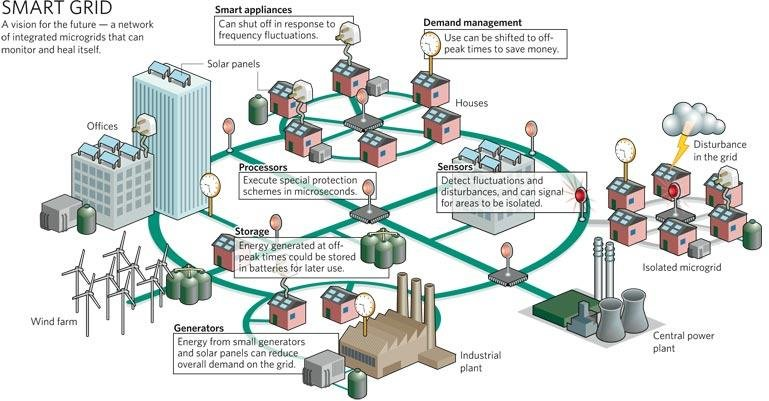
\includegraphics[width = \textwidth]{smartgrid.jpg}\\
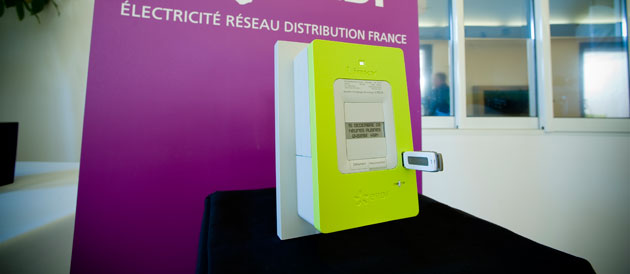
\includegraphics[width = \textwidth]{linky.jpg} 

\end{columns}

\end{frame}

\begin{frame}{Des données variées, à différentes échelles}

\begin{figure}[!ht] \centering
  \begin{minipage}[c]{0.48\textwidth}
     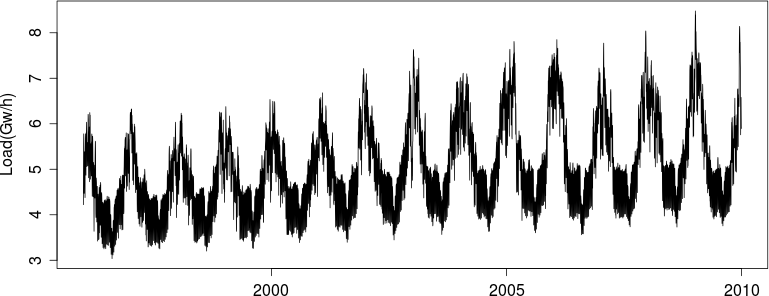
\includegraphics[width=\textwidth,height=3.45cm]{longtermload.png}
     \vspace*{-0.35cm}
%     \vspace*{-0.85cm}
     \caption{Tendance à long terme} %\label{fig:gull}
  \end{minipage}%
  ~ %spacing between images
  \begin{minipage}[c]{0.48\textwidth}
     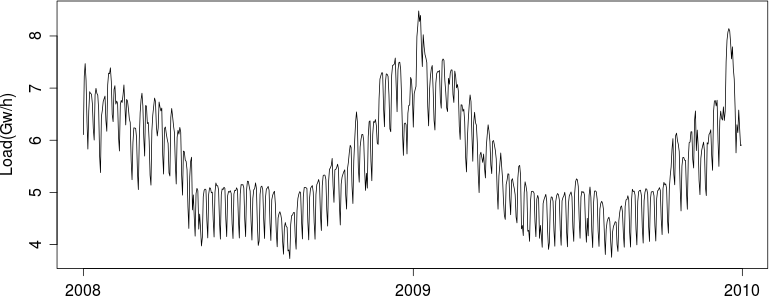
\includegraphics[width=\textwidth,height=3.45cm]{twoyearsload.png}
     \vspace*{-0.35cm}
%     \vspace*{-0.85cm}
     \caption{Cyclicité semaine} %     \label{fig:tiger}
  \end{minipage}
  ~\\[-0.05cm]
  \begin{minipage}[c]{0.48\textwidth}
     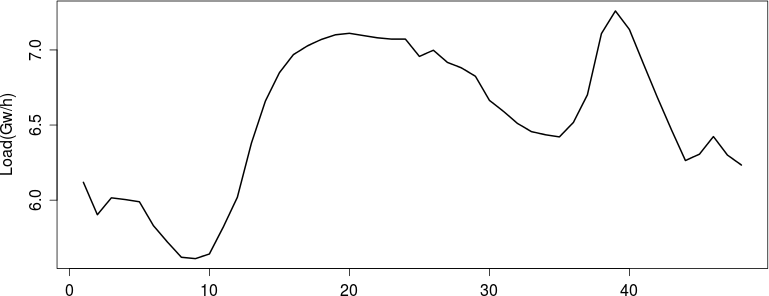
\includegraphics[width=\textwidth,height=3.45cm]{dailyloads.png}
     \vspace*{-0.35cm}
%     \vspace*{-0.85cm}
     \caption{Moyenne journalière} %   \label{fig:mouse}
  \end{minipage}
  ~ %spacing between images
  \begin{minipage}[c]{0.48\textwidth}
     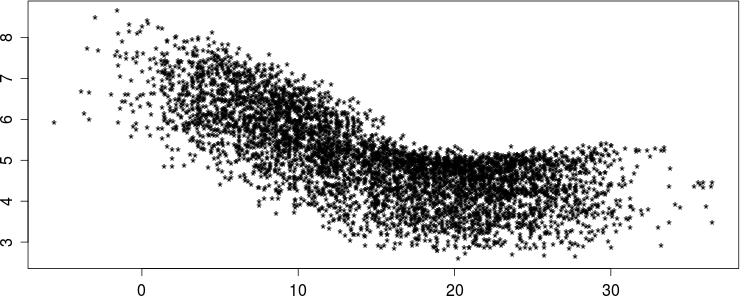
\includegraphics[width=\textwidth,height=3.45cm]{consotemp.png}
     \vspace*{-0.35cm}
%     \vspace*{-0.85cm}
     \caption{Conso. vs. température}
  \end{minipage}
\end{figure}

\end{frame}

\begin{frame}{Découpage en tranches non stationnaires}

Si $\exists \delta \ll D$, tel que les séries $\delta-$agrégées soient stationnaires,\\
on les agrège et les traite comme des processus stationnaires.\\[0.3cm]

\begin{columns}
  \column{6cm}    
      \begin{tikzpicture}[scale=0.5]
 
     % Axis
     \draw[<->, thick] (0,4) node (yaxis) [left] {$X_t$} 
        |- (11,0) node (xaxis) [right] {$t$} ;
     % Dashed grid
     \foreach \t in {1, 2, 3, 4, 5, 6} 
        \draw[dashed, color=PineGreen] (1.5*\t cm, 4) -- (1.5*\t cm, -3pt) 
                         node[anchor=north] {$\t \delta$};

     \draw[color=PineGreen] plot[smooth] file {tikz/data.dat};

     \draw (0,0) -- (0,-3pt) node[below, color= PineGreen] {0};
     \draw[dashed, color=PineGreen] (1.5*7,4) -- (1.5*7,-3pt) 
                         node[below] {};%$T+\delta$

     \foreach \t in {1, 2, 5} 
        \draw[color=PineGreen] (-0.75+1.5*\t, 1.5) node[below, scale=0.75] {$Z_\t(t)$};
        
     \foreach \t in {3, 4, 6} 
        \draw[color=PineGreen] (-0.75+1.5*\t, 3.5) node[below, scale=0.75] {$Z_\t(t)$};
     
  \end{tikzpicture} 

   ~
  \column{5cm}
	\vspace*{-1cm}
     \[ Z_k(t) = X(t + (k-1)\delta)             \]
     \[  k\in\N \;\;\; \forall t \in [0,\delta) \]
\end{columns}

\textbf{\emph{Mais...}} 
Une série temporelle représentant un phénomène complexe 
\textcolor{white}{\textbf{\emph{Mais...}} }est en général clairement non stationnaire.\\[0.5cm]

$\Rightarrow$ On décide de tenir compte de chaque point de discrétisation.

%Par exemple, la consommation électrique moyenne sur une semaine varie

%~ \vfill
  %~ If $X$ contents a $\delta-$seasonal component, 
     %~ $Z$ is particularly fruitful.

%~ C'est pas vraiment notre cas : saisonnier à plusieurs echelles
%~ ==> objectif : tout prendre en compte

\end{frame}

\begin{frame}{Réduction de dimension}

Données enregistrées toutes les 30 minutes pendant un an :\\
$48 \times 365 =$ \textbf{17520 points de discrétisation}.\\[0.3cm]

\vspace*{-0.4cm}
\begin{figure}[!ht]
\centering
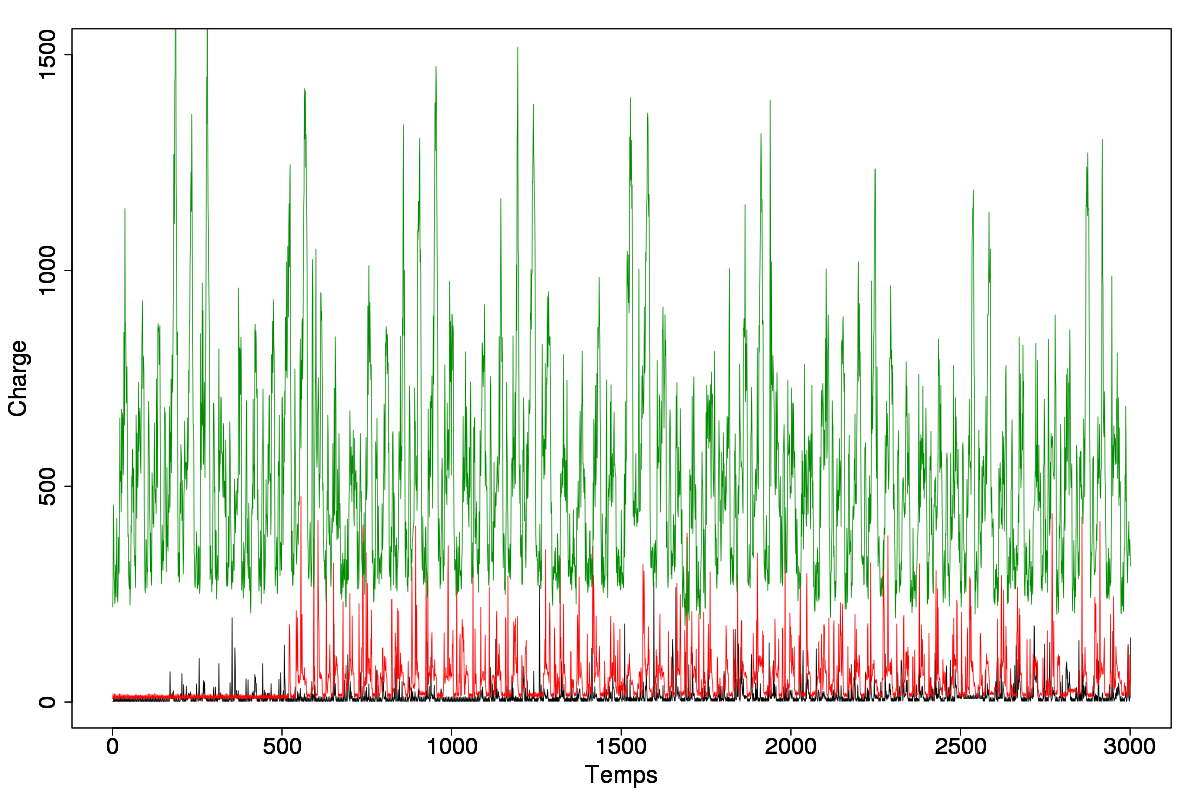
\includegraphics[width=\textwidth,height=5.5cm]{3centers.png}
\vspace*{-0.35cm}
%\vspace*{-0.95cm}
\caption{Trois types de courbes de charge \emph{(données irlandaises)}}% présentant différents régimes}%{[Spoiler] Cinq centres de clusters}
\end{figure}

\vspace*{-0.3cm}
$\Rightarrow$ Il faut déterminer une représentation parcimonieuse, capturant\\
\textcolor{white}{$\Rightarrow$ }bien les variations localisées. On choisit une base d'ondelettes.\\[0.5cm]
%TODO: placer l'equation puis sa version discrète.

\end{frame}

\begin{frame}{Wavelets to cope with \textsc{fd}}

\begin{columns}
  \column{.6\textwidth}
 %\begin{figure}
 \centering
 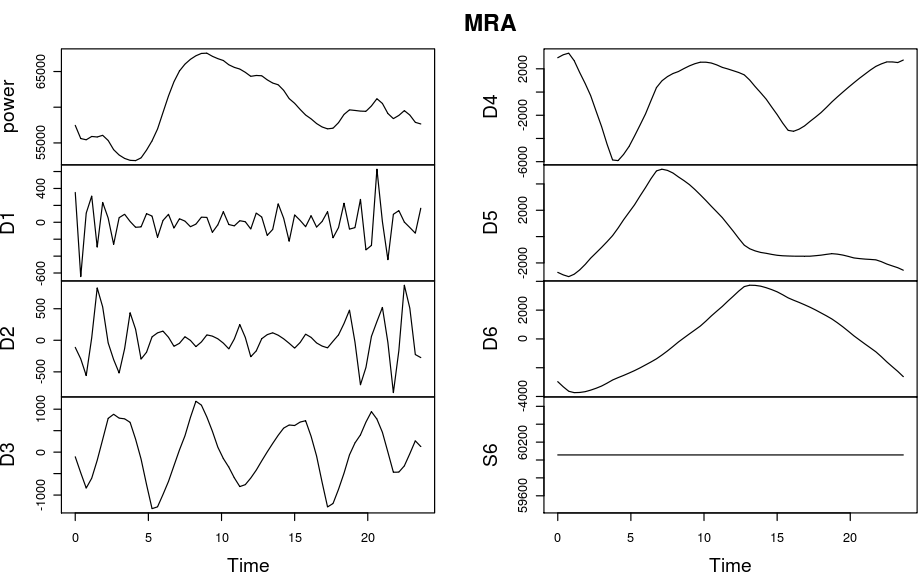
\includegraphics[width = \textwidth]{./pics/weekly-5.png}
  % * * * * * * * *  * * * * * * * * * * *
  \column{.4\textwidth}
\begin{footnotesize}
\begin{itemize}
 \item domain-transform technique for hierarchical decomposing finite energy signals
 \item description in terms of a broad trend (\textcolor{PineGreen}{approximation part}), plus a set of localized changes kept in the \textcolor{red}{details parts}.
\end{itemize}
\end{footnotesize}
\end{columns}

\vspace*{-0.1cm}
\begin{block}{Discrete Wavelet Transform }
\begin{footnotesize}
  If $z \in L_2([0, 1])$ we can write it as
  \vspace*{-0.4cm}
   \begin{equation*}\label{eq:zeta}
     z(t) = \sum_{k=0}^{2^{j_0}-1} \textcolor{PineGreen}{c_{j_0, k}} \phi_{j_0,k} (t)  + 
        \sum_{j={j_0}}^{\infty} 
           \sum_{k=0}^{2^j-1} \textcolor{red}{d_{j,k}} \psi_{j,k} (t) ,
   \end{equation*}
%
~\\[-0.6cm]
where $ c_{j,k} = <g, \phi_{j,k} > $, $ d_{j,k} = <g, \varphi_{j,k}>$ are the 
\textcolor{PineGreen}{scale coefficients} and \textcolor{red}{wavelet coefficients} respectively, and the functions $\phi$ et $\varphi$ are associated to a orthogonal \textsc{mra} of $L_2([0, 1])$.
\end{footnotesize}
\end{block}
\end{frame}

%---------------------------------------- SLIDE ---------------------

\begin{frame}{Energy decomposition of the DWT}

\begin{block}{ }
 \begin{itemize}
  \item Energy conservation of the signal
\vspace*{-0.15cm}
  \begin{equation*}\label{eq:energy}  
     \| z \|_H^2    \approx     \| \widetilde{z_J} \|_2^2 
        = c_{0,0}^2 + \sum_{j=0}^{J-1} \sum_{k=0}^{2^j-1} d_{j,k} ^2  = 
                     c_{0,0}^2 + \sum_{j=0}^{J-1} \| \mathbf{d}_{j} \|_2^2.
  \end{equation*}
%  \item characterization by the set of channel variances estimated at the output of the corresponding filter bank
 \item For each $j=0,1,\ldots,J-1$, we compute the absolute and 
 relative contribution representations by
\vspace*{-0.15cm}      
   \[ \underbrace{\hbox{cont}_j = ||\mathbf{d_j}||^2}_{\fbox{AC}}  
      \qquad  \text{and}  \qquad
       \underbrace{\hbox{rel}_j  = 
     \frac{||\mathbf{d_j}||^2}
          {\sum_j ||\mathbf{d_j}||^2 }}_{\fbox{RC}} .\]
 \item They quantify the relative importance of the scales to the global dynamic.
% \item Only the wavelet coefficients $\set{d_{j,k}}$ are used.
 \item RC normalizes the energy of each signal to 1.
\end{itemize}
\end{block}
\end{frame}

%===========================================================================================
% fin de l'intro...
%===========================================================================================

\begin{frame}{Objectif}

\begin{figure}[!ht]\centering
  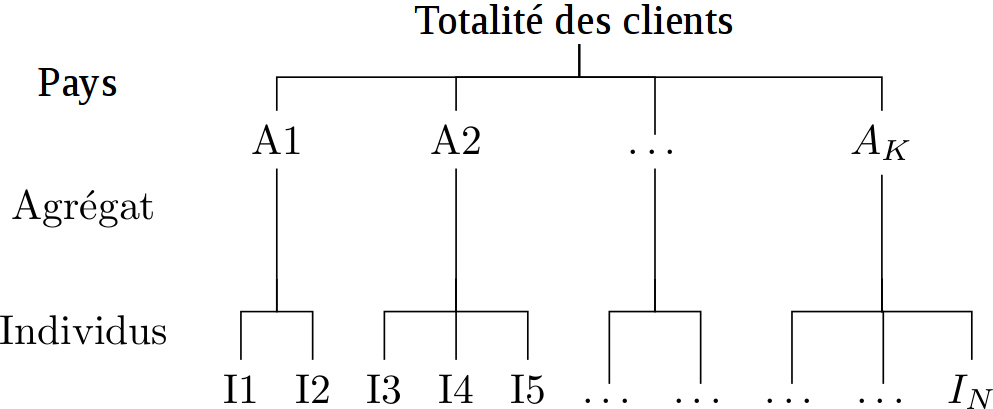
\includegraphics[width = \textwidth]{pics/schema.png} 
%\caption{Hierarchical structure of $N$ individual clients among $K$ groups.}\label{fig:schema-hier}
\end{figure}

Regroupement par tarifs, zones géographiques, types de clients \dots\\[0.3cm]

$\Rightarrow$ \textbf{Idée} : clustering pour déterminer ces groupes.\\[0.3cm]

\textcolor{white}{$\Rightarrow$ }\textbf{Méthode} : paralléliser un algorithme classique.

%~ functional clustering
%~ wavelets to reduce dimension
%~ open MPI to cluster a bounded number of vectors at a time

\end{frame}

\begin{frame}{Fonction objectif}

On cherche à minimiser la distorsion
$$\Delta = \sum_{i=1}^{n} \min_{k=1..K} \| x_i - c_k \|_2^{}$$
avec pour variables les $\{c_1,\dots,c_K\} \subset \{x_1,\dots,x_n\}, c_i \neq c_j \,  \forall i \neq j$.\\[0.3cm]

C'est un problème NP-dur {\footnotesize (O. Kariv \& S. L. Hakimi, \emph{An Algorithmic Approach to Network Location Problems. II: The p-Medians})}.\\[0.1cm]
%SIAM J. Appl. Math., 37(3), 539–560. (22 pages)
%~ C'est-à-dire :
%~ \begin{itemize}
%~ \item Soit $P$ le problème de décision associé : $P(c_1,\dots,c_k) = 1$ si $(c_1,\dots,c_k)$ est optimal, 0 sinon.
%~ \item Soit $C$ un problème de décision bien connu comme étant NP-complet
%~ \item Il existe un algorithme ...
%~ \end{itemize}

Pire : garantir un facteur $(1+\varepsilon)$ de l'optimum est NP-dur 
{\footnotesize (J-H. Lin \& J. S. Vitter $\varepsilon$-Approximations with Minimum Packing Constraint Violation)}.\\[0.2cm]%(Extended Abstract)

\begin{block}{NP : ``Non-deterministic Polynomial-time algorithms''}
{\footnotesize Exécution en temps polynomial sur une machine de Turing non déterministe.}
\end{block}

\begin{block}{NP-dur}
``Au moins aussi dur que le plus complexe des problèmes NP''
\end{block}

%~ Tous les algorithmes existants déterminant les $c_k$ sont donc des heuristiques d'approximation
%~ ...et parler de la parallélisation ??! donc 16 slides au total.
%NP-complet : c'est à dire... expliquer.
%Algos existants = heuristiques pr s'approcher de l'optimum (d'un...)

\end{frame}

\begin{frame}{Algorithme PAM}

%PAM : montrer algo, dire comment on parallélise naïvement

\begin{enumerate}
\setcounter{enumi}{-1}
\item Initialize: randomly select (without replacement) $K$ of the $n$ data points as the medoids.
\item Associate each data point to the closest medoid. (``closest'' here is defined using any valid distance metric, most commonly Euclidean distance, Manhattan distance or Minkowski distance).
\item For each medoid $m$\\
\quad For each non-medoid data point $o$ \emph{in the same cluster}\\
\quad\quad Swap $m$ and $o$ and compute the total cost.
\item Select the configuration with the lowest cost.\\
If any change occurred in the medoids, go to step 1.
\end{enumerate}

\begin{block}{Réduire le coût des étapes 2 et 3 ?}
\begin{itemize}
\item Dans R, pam(do.swap=FALSE) supprime les étapes 2 et 3.
\item A. P. Reynolds et al. (2006) : quelques astuces algorithmiques.
\end{itemize}
\end{block}

\end{frame}

\begin{frame}{Parallélisation}

\begin{block}{Deux approches (entre autres)}
\begin{itemize}
\item Découpage de l'espace en $Z < K$ zones, et recherche de $K/Z$ clusters dans chaque zone.
\item Partition des données $P_1,\dots,P_Z$ puis clustering à $K$ groupes dans chaque $P_k$. 
(Puis ``fusion'' des médoïdes).
\end{itemize}
\end{block}

~\\[-0.1cm]
{\footnotesize
Choix de la seconde alternative et implémentation avec OpenMPI :
\begin{enumerate}
\setcounter{enumi}{-1}
\item Le processus ``maître'' a pour numéro 0. Il divise les données en sous-ensembles de cardinal au plus 
$C$ ($C = 5000$ par exemple). Il envoie ensuite une tâche de clustering par sous-ensemble, et attend les résultats.
\item Chaque processus ``esclave'' (numérotés de 1 à $p-1$) reçoit une liste de (références de) courbes, qu'il récupère 
et classe via l'algorithme PAM. Il retourne les centres au processus 0.
\item Si on obtient plus de $C$ médoïdes, on recommence depuis l'étape 1. Sinon, on applique une dernière 
fois l'algorithme PAM (sur les médoïdes).
\end{enumerate}
}

\end{frame}

\begin{frame}{Exécution du programme}

\vspace*{-0.5cm}
\begin{figure}
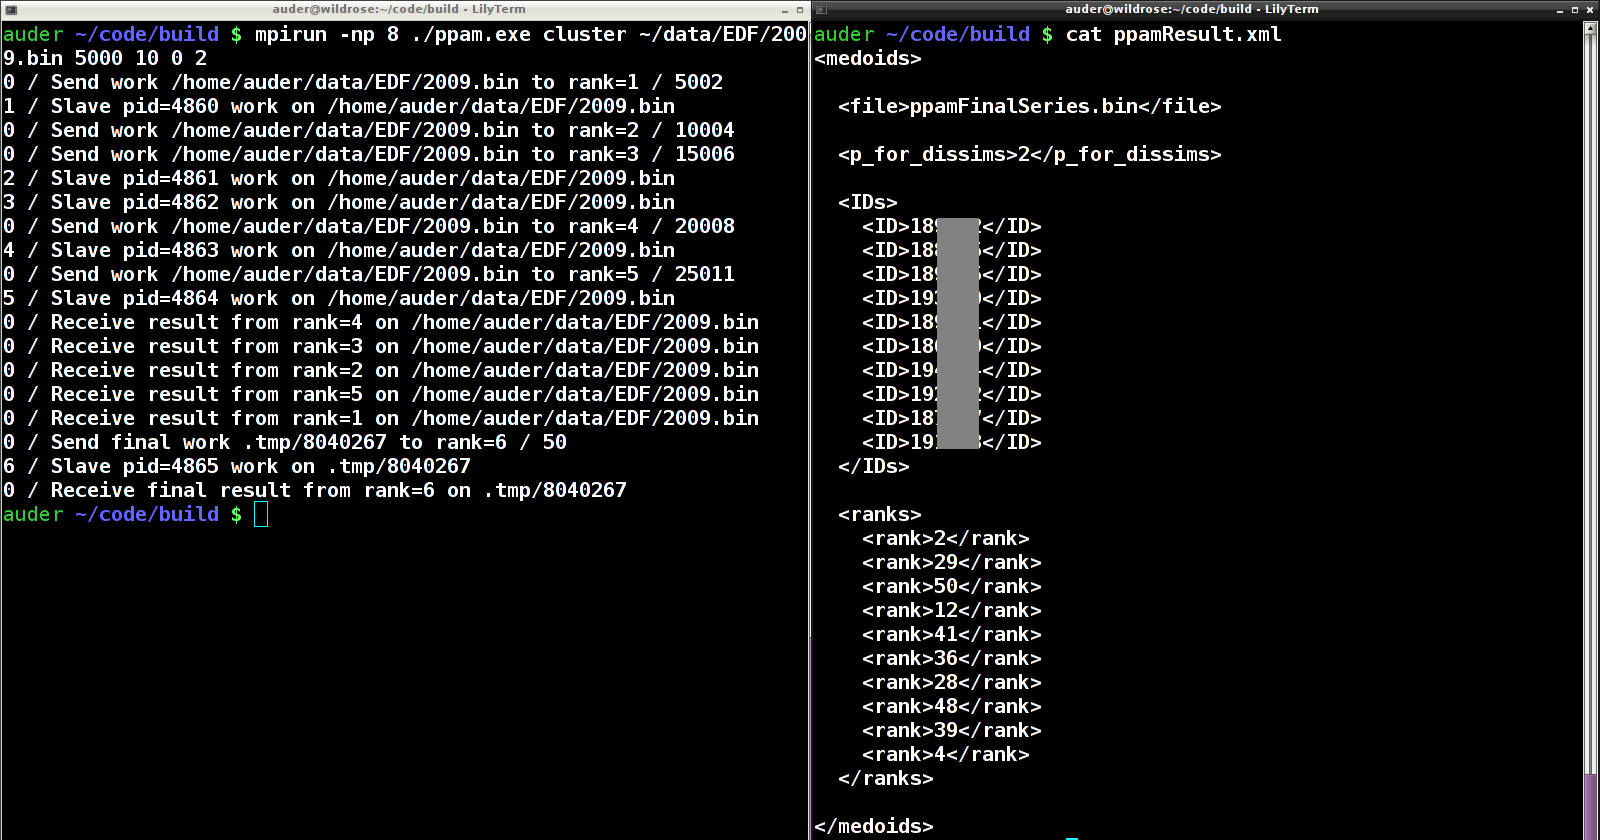
\includegraphics[width=\linewidth,height=8cm]{pics/screen_demo.png}
	%~ \vspace*{-0.35cm}
	%~ \caption{Groupe 1}
\end{figure}

\end{frame}

\begin{frame}{Application I: Electricity Smart Meter CBT}

%\footnotetext[1]{\textit{Irish Social Science Data Archive}, }

\begin{itemize}
 \item 4621 Irish households smart meter data 
 (\href{http://www.ucd.ie/issda/data/}{ISSDA})
 % eséries de consommation électrique de foyers irlandais
 \item About 25K discretization points 
 \item We test with $K=$ 3 or 5 classes
 \item We compare sequential and parallel versions 
\end{itemize}

\begin{table}[H]
\centering
\begin{tabular}{lcc}                       \hline
% &            &       \\
 & Distortion & (Internal) adequacy  \\ \hline
3 clusters sequential & 1.90e7 & 0.90   \\
3 clusters parallel   & 2.15e7 & 0.90   \\
5 clusters sequential & 1.61e7 & 0.89   \\
5 clusters parallel   & 1.84e7 & 0.89   \\ \hline
\end{tabular}
%  \caption{Distorsions et indices d'adéquation des partitions}
\end{table}

\textbf{Adequacy :} given $P_1 = (i_1,\dots,i_n)$ and $P_2 = (j_1,\dots,j_n)$,\\
\textcolor{white}{\textbf{Adequacy :}} find a matching which maximize $S = \sum_{k=1}^{n} \mathbb{1}_{i_k = j_k}$\\
\textcolor{white}{\textbf{Adequacy :}} (hungarian algorithm), and then return $S/n$.

\end{frame}

\begin{frame}{Application II: Starlight curves}

\begin{itemize}
 \item Data from \href{http://www.cs.ucr.edu/~eamonn/time_series_data/}{UCR Time Series Classification/Clustering}
 %\url{http://www.cs.ucr.edu/~eamonn/time_series_data/}}
 \item 1000 curves learning set + 8236 validation set ($d = 1024$)% discretization points
\end{itemize}

\begin{figure}[H]
\begin{minipage}[c]{.32\linewidth}
	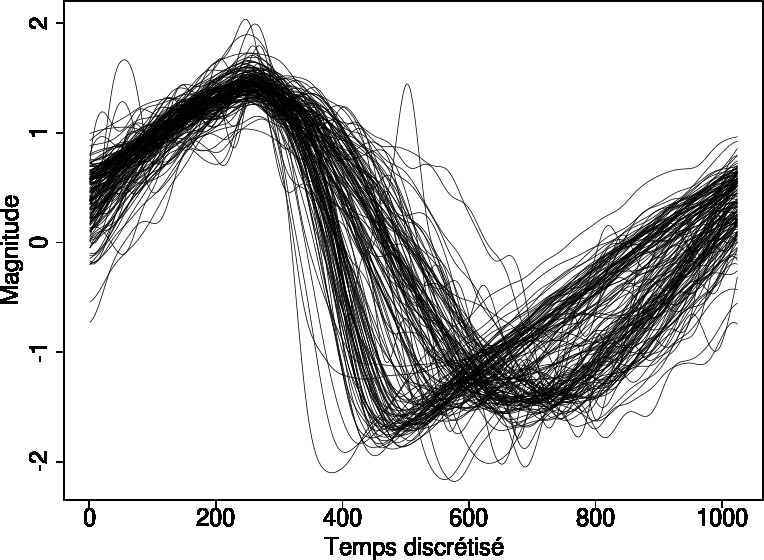
\includegraphics[width=\linewidth,height=3.5cm]{pics/slgr1.png}
	\vspace*{-0.35cm}
	\caption{Groupe 1}
\end{minipage}
\begin{minipage}[c]{.32\linewidth}
	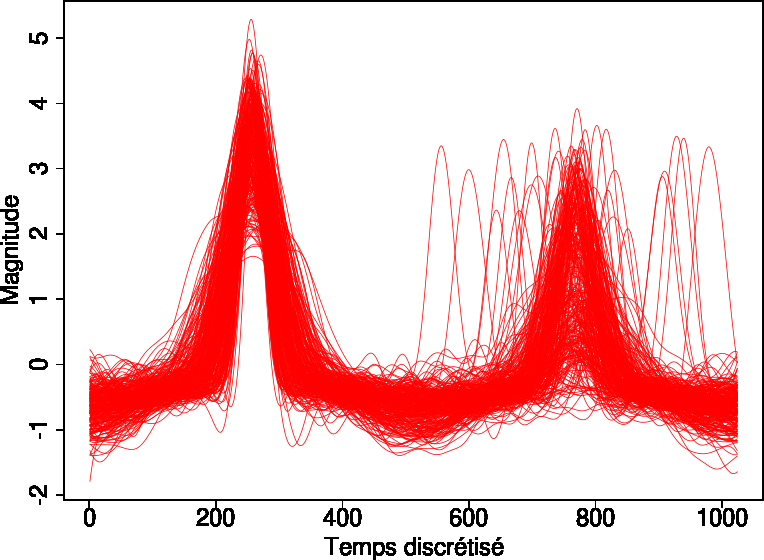
\includegraphics[width=\linewidth,height=3.5cm]{pics/slgr2.png}
	\vspace*{-0.35cm}
	\caption{Groupe 2}
\end{minipage}
\begin{minipage}[c]{.32\linewidth}
	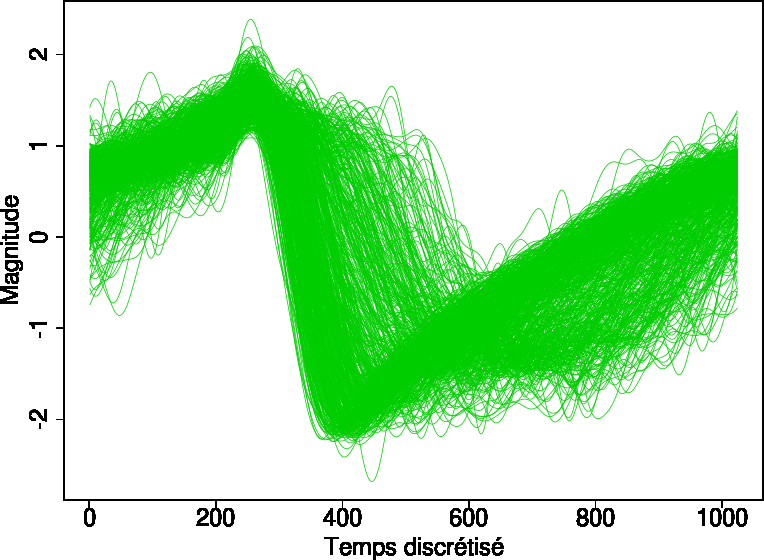
\includegraphics[width=\linewidth,height=3.5cm]{pics/slgr3.png}
	\vspace*{-0.35cm}
	\caption{Groupe 3}
\end{minipage}
\end{figure}

\begin{footnotesize}
\vspace*{-0.3cm}
\begin{table}[H]
\centering
\begin{tabular}{lccc}                           \hline
 &            & \multicolumn{2}{c}{Adequacy} \\
 & Distortion & Internal & External          \\ \hline
Training (sequential) & 1.31e4 & 0.79 & 0.77 \\
Training (parallel)   & 1.40e4 & 0.79 & 0.68 \\
Test (sequential)     & 1.09e5 & 0.78 & 0.76 \\
Test (parallel)       & 1.15e5 & 0.78 & 0.69 \\ \hline
\end{tabular}
%\caption{Distorsions et indices d'adéquation des partitions}
\end{table}
\end{footnotesize}

\end{frame}

\begin{frame}{Conclusion}

%~ On peut clusteriser
%~ Faudrait etre moins naif
%~ Faudrait aussi étendre/généraliser le code...

\begin{block}{Résumé}
\begin{itemize}
\itemsep0.1em
\item Les smartmètres mesurent la charge électrique pour chaque client, en temps réel $\Rightarrow$ données fonctionnelles.
\item Les ondelettes fournissent des représentations parcimonieuses tout en préservant la nature fonctionnelle des données.
\item L'analyse de ces représentations à l'aide de l'algorithme PAM permet d'identifier des groupes de clients.
\item L'algorithme PAM est appliqué en parallèle sur des jeux de données de tailles raisonnables.
\end{itemize}
\end{block}

% \item \textit{Divide-and-Conquer} approach thanks to MPI library %pour l'algorithme des $k$-médoïdes : d'abord  sur des groupes de données courbes, puis des groupes de médoïdes jusqu'à obtenir un seul ensemble traité sur un processseur.
 %\item %Les résultats obtenus sur les deux jeux de données présentés sont assez encourageants, et permettent d'envisager une utilisation à plus grande échelle.
%\end{itemize}

\begin{exampleblock}{Perspectives}
\begin{itemize}
\itemsep0.1em
\item L'étude des groupes de clients peut donner lieu à l'élaboration de $K$ modèles prédictifs spécialisés.
\item La méthode de clustering parallèle proposée peut être adaptée pour traiter les 35M séries (sur un supercalculateur ?).
%\item Apply the algorithm over many hundreds of processors
\end{itemize}
\end{exampleblock}

\end{frame}

\begin{frame}{Références}

\begin{thebibliography}{4}
\bibitem{1} \textcolor{black}{A. Antoniadis, X. Brossat, J. Cugliari, J.-M. Poggi} (2013), Clustering Functional Data Using Wavelets, \textcolor{black}{{\it Wavelets, Multiresolution and Information Processing}, 11(1), 35--64}

\bibitem{2} \textcolor{black}{A. Arbelaez, L. Quesada} (2013), Parallelising the k-Medoids Clustering Problem Using Space-Partitioning, \textcolor{black}{{\it Symposium on Combinatorial Search}, AAAI Publications}

\bibitem{3} \textcolor{black}{R. Bekkerman, M. Bilenko, J. Langford - éditeurs} (2011), 
Scaling up Machine Learning: Parallel and Distributed Approaches, \textcolor{black}{Cambridge University Press}

\bibitem{4} \textcolor{black}{A. P. Reynolds, G. Richards, B. de la Iglesia, V. J. Rayward-Smith} (2006), Clustering Rules: A Comparison of Partitioning and Hierarchical Clustering Algorithms, \textcolor{black}{{\it Mathematical Modelling and Algorithms}, 5(4), 475--504}

%\bibitem{3} P. Berkhin (2006), A Survey of Clustering Data Mining Techniques, {\it Grouping Multidimensional Data, éditeurs : J. Kogan, C. Nicholas, M. Teboulle}.

%\bibitem{6} J. Dean et S. Ghemawat (2004), MapReduce: Simplified Data Processing on Large Clusters, {\it Sixth Symposium on Operating System Design and Implementation}.

%\bibitem{7} G. De Francisci Morales et A. Bifet (2013), G. De Francisci Morales SAMOA: A Platform for Mining Big Data Streams Keynote Talk at RAMSS ’13: 2nd International Workshop on Real-Time Analysis and Mining of Social Streams WWW, Rio De Janeiro

%\bibitem{10} L. Kaufman et P.J. Rousseeuw (1987), Clustering by means of Medoids, {\it Statistical Data Analysis Based on the L\_1-Norm and Related Methods, éditeur : Y. Dodge}.
\end{thebibliography}

%[2013] A. Antoniadis, X. Brossat, J. Cugliari & J.-M. Poggi. Clustering functional data using Wavelets Inter. J. of Wavelets, Multiresolution and Information Procesing. doi:10.1142/S0219691313500033

%~ Scaling up Machine Learning: Parallel and Distributed Approaches [Anglais] [Relié]
%~ Ron Bekkerman (Sous la direction de), Mikhail Bilenko (Sous la direction de), John Langford

\end{frame}

\begin{frame}

\centering

\includegraphics[width=7cm,height=7cm]{Questions.jpg}

\end{frame}

\end{document}
